\documentclass[11pt,a4paper]{report}
\usepackage[french]{babel}
\usepackage[utf8]{inputenc}
\usepackage[T1]{fontenc}
\usepackage{layout}
\usepackage{titlesec}
\usepackage{lmodern}
\usepackage{enumitem}
\usepackage{amsmath}
\usepackage{empheq}
\usepackage{amssymb}
\usepackage{mathrsfs}
\usepackage{array}
\usepackage{gensymb}
\usepackage{mathenv}
\usepackage{color, colortbl}
%\usepackage[intlimits]{amsmath}
\usepackage[usenames,dvipsnames]{xcolor}
\usepackage{listings}
\usepackage{graphicx}
\usepackage{fancybox}
\usepackage{fourier-orns}



\definecolor{codecustom}{rgb}{0,0.5,0}
\definecolor{codegray}{rgb}{0.7,0.7,0.7}
\definecolor{codepurple}{rgb}{0.58,0,0.82}
\definecolor{backcolour}{rgb}{0.975,0.97,0.975}
\definecolor{custom}{RGB}{216,0,127}
\definecolor{lightgray}{gray}{0.75}
\definecolor{myblue}{rgb}{.8, .8, 1}
\definecolor{redcustom}{RGB}{255,0,0}

\titleformat{\chapter}[hang]{\bf\huge}{\thechapter}{2pc}{}


\usepackage[final]{pdfpages} %inclure un pdf


  \newcommand*\mybluebox[1]{%
    \colorbox{myblue}{\hspace{0.5em}#1\hspace{1em}}}

\lstdefinestyle{mystyle}{
	language=MATLAB,
    backgroundcolor=\color{backcolour},
    commentstyle=\color{codecustom},
    keywordstyle=\color{custom},
    morekeywords={Fe, Te, sin, carre, Liste, ELEMENT},
    numberstyle=\tiny\color{codegray},
    stringstyle=\color{codepurple},
    basicstyle=\footnotesize,
    breakatwhitespace=false,
    breaklines=true,
    captionpos=t,
    keepspaces=true,
    numbers=left,
    numbersep=5pt,
    showspaces=false,
    showstringspaces=false,
    showtabs=false,
    tabsize=2,
    extendedchars=true,
    literate={é}{{\'e}}1 {Ú}{{\`e}}1 {Ã}{{\`a }}1 {ç}{{\c{c}}}1 {œ}{{\oe}}1 {ÃŜ}{{\`u}}1
{É}{{\'E}}1 {È}{{\`E}}1 {À}{{\`A}}1 {Ç}{{\c{C}}}1 {Œ}{{\OE}}1 {Ê}{{\^E}}1
{ê}{{\^e}}1 {î}{{\^i}}1 {ÃŜ}{{\^o}}1 {û}{{\^u}}1 {â}{{\^a}}1,
}

\lstset{style=mystyle}

\frenchbsetup{StandardItemLabels=true, CompactItemize=false, ReduceListSpacing=true}
\setcounter{tocdepth}{4}
\usepackage{caption}
\DeclareCaptionFont{white}{\color{white}}
\DeclareCaptionFormat{listing}{\colorbox{codecustom}{\parbox{\textwidth}{#1#2#3}}}
\captionsetup[lstlisting]{format=listing,labelfont=white,textfont=white}

\renewcommand{\lstlistingname}{Code Extracted}

%%%%%%%% Espace entre paragraphe et Indentation %%%%%%%%%%%%%%%%%%%%

\setlength{\parskip}{0.09cm}
\setlength{\parindent}{0.8cm}

%%%%%%%%%%%%%%%%%%%%%%%%%%%%%%%%%%%%%%%%%%%%%%%%%%%%%%%%%%%%%%%%%%%%


%%%%%%%%%%%%%%%%%%%%%% Dimensions de la page %%%%%%%%%%%%%%%%%%%%%%%%%

\usepackage[top=2cm, bottom=2cm, left=2cm, right=2cm]{geometry}

%%%%%%%%%%%%%%%%%%%%%%%%%%%%%%%%%%%%%%%%%%%%%%%%%%%%%%%%%%%%%%%%%%%%%%

%%%%%%%%%%%%%%%%%%%% Lien Hyperref Sommainre %%%%%%%%%%%%%%%%%%%%%%%%%%


\usepackage{hyperref} % Créer des liens et des signets

%%%%%%%%%%%%%%%%%%%%%%%%%%%%%%%%%%%%%%%%%%%%%%%%%%%%%%%%%%%%%%%%%%%%%%

%%%%%%%%%%% Gestion des en-tête/pieds de page %%%%%%%%%%%%%%%%%%%%%%%%%%%

\usepackage{fancyhdr}
\pagestyle{fancy}

% Permet d'écrire le nom des chapitres et section en minuscules au lieu de majuscules definit par défaut
\renewcommand{\chaptermark}[1]{\markboth{\bsc{\chaptername~\thechapter{} :} #1}{}}
\renewcommand{\sectionmark}[1]{\markright{\thesection{} #1}}
%

\renewcommand{\headrulewidth}{0.4pt} % epaisseur du trait
\fancyhead[C]{}
\fancyhead[L]{\leftmark}
\fancyhead[R]{Guedira}

\renewcommand{\footrulewidth}{0.4pt}
\fancyfoot[C]{\textbf{Page \thepage}}
%\fancyfoot[L]{}
%\fancyhead[C]{}
\fancyhead[R]{\leftmark}
\fancyhead[L]{}

\renewcommand{\footrulewidth}{0.4pt}
\fancyfoot[C]{\textbf{Page \thepage}}
\fancyfoot[L]{\textsc{Ismail Guedira}}
\fancyfoot[R]{\rightmark}

%%%%%%%%%%%%% Option des annexes %%%%%%%%%%%%%%%%%%%%%%%%%%%

\usepackage[toc,page]{appendix}
\renewcommand{\appendixtocname}{Annexes}
\renewcommand{\appendixpagename}{Annexes}
\renewcommand{\appendixname}{Annexes}
%%%%%%%%%%%%%%%%%%%%%%%%%%%%%%%%%%%%%%%%%%%%%%

\newcommand{\gray}{\rowcolor[gray]{.90}}

\usepackage{pifont} %utiliser des signes pour les itemize plutot cool

\usepackage{lscape}	%pouvoir passer en mode paysage



%%%%%%%%%% Change le nom Table en Tableau %%%%%%%%%%

% \addto\captionsfrench{\def\tablename{Tableau}}

%@\addto\captionsfrench{\def\figure{Figure}}

\title{Semester Project -- Bandgap Reference Voltage}
\author{Ismail Guedira}
\usepackage{layout}



\begin{document}


%%%%% %%%%%%%%%                       Et si on refaisait la page de garde            %%%%%%%%%%%%%%%%%%%%%%%%%%%%%%

 \makeatletter
   \begin{titlepage}
  % \centering
    {
    
    
    \Large \textbf{EPFL - Microcity} \hfill \\
    \large \textsc{Rue de la Maladière 71,} \hfill \\ %Rue de la Maladière 71, 2000 Neuchâtel
	  \large \textsc{2000 Neuchatel} \hfill \\
    \large \textsc{SUISSE} \hfill \\ }
    \begin{flushright}
      
\includegraphics[height=0.1\textheight]{logo_epfl} 
    \end{flushright}
    
	\hspace{3em}
% 
% 
% \hfill \Large   \textsc{\@author} \hfill \\ 
% \hfill \normalsize \bfseries Exchange Student EPFL \\
% \hfill \normalsize \it Génie Électrique et électronique \\ 
 \vfill
\centering

 
     \hrule
    %  \vspace{2em}
    %  \LARGE \textbf{} \\
     \vspace{2em}
     \huge \textbf{\@title} \\
     \vspace{1em}
     \LARGE \textit{ESPLAB - Electronic and Signal Processing Laboratory}
     \vspace{2em}
     \hrule
    
        
    
%  \hfill   \large $2^{ième}$ Année - \textbf{S}ystèmes \textbf{É}lectroniques \textbf{I}ntégrés \hfill \\
%  \hfill   \textit{ismail.guedira@phelma.grenoble-inp.fr} \hfill \\
% 	\vspace{2em}
% 
%     % \Large \textbf{Maitre de Stage :} 	\hfill	\Large \textsc{Hugo Petit} \\
%    % 										\hfill	\large \textbf{Analog Design Manager} \\
%    % 										\hfill	\textit{hugo.petit.cn@rolls-royce.com} \\
% 
% 
     \vfill
% 
      {\Large \textsc{2014/2015}  \hfill \Large \textsc{\@date}} \\
% 
% 
  \end{titlepage}
\makeatother

%%%%%%%%%%%%%%%%%%%%%%%%%%%%%%%%%%%%%%%%%%%%%%%%%%%%%%%%%%%%%%%%%%%%%%%%%%%%%%%%%%%%%%%%%%%%%%%%%%%%%%%%%%%%%%%%%%%

%\maketitle
\pagenumbering{roman}
\renewcommand{\contentsname}{Sommaire}
\tableofcontents


% \newpage
% \chapter*{Remerciement}
% \addcontentsline{toc}{chapter}{Remerciement}
% 
% REMERCIEMENT
% 
% 
% \chapter*{Introduction}
% \addcontentsline{toc}{chapter}{Introduction}
% 
% INTRODUCTION
% 

\newpage
% 
\addcontentsline{toc}{chapter}{Abstract}
\vspace{3cm}
\textbf{Abstract} \\
\newline
\hspace*{17pt} ABSTRACT

\newpage
\begin{minipage}{\textwidth}
  \listoffigures
  \listoftables
\end{minipage}

\newpage

\pagenumbering{arabic}

\chapter{Principle \& Specifications}

Voltage references have always been an essential component of any system and consequently an important topic to explore. The last decades thrust toward higher and even total system integration has required all designers to be knowledgeable of this particular topic due to its mixed-signal implications (output impedance, temperature coefficient, etc...)


A general-use (ideal) voltage reference is a circuit used to generate a fixed voltage, $V_{ref}$, that is independent of the power supply voltage VDD (where $V_{ref} < VDD$ ), temperature, and process variations. In other words, the ideal reference voltage is independent of PVT. In some cases, we want to design a reference that varies with temperature. For example, if $V_{ref}$ increases with temperature, Fig. \ref{ptat_crb}, we say that the reference voltage is proportional to absolute temperature or \textbf{PTAT}. If the reference voltage decreases with increasing temperature,            Fig. \ref{CTAT_crb}, the reference is said to be complementary to absolute temperature or \textbf{CTAT}. 

\begin{figure}[h!]
   \begin{minipage}[b]{0.5\linewidth}
      \centering 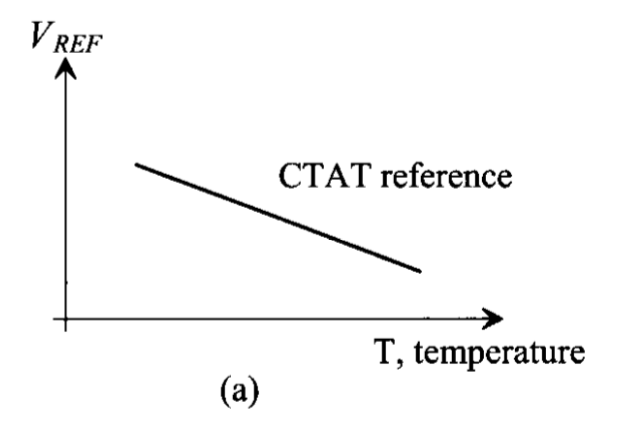
\includegraphics[scale=0.4]{photo/CTAT_crb}
      \caption{CTAT Voltage Evolution}
      \label{CTAT_crb}
   \end{minipage}\hfill
   \begin{minipage}[b]{0.5\linewidth}
      \centering 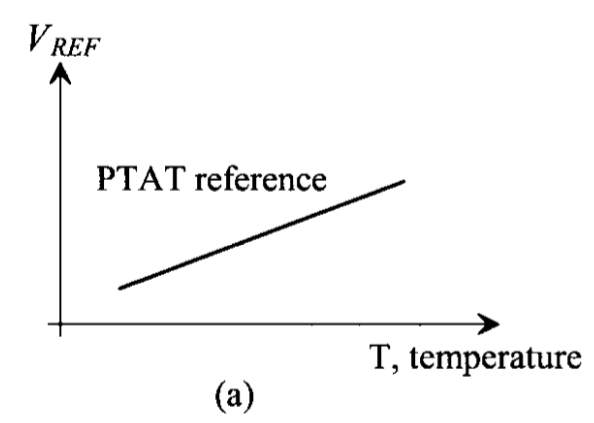
\includegraphics[scale=0.4]{photo/PTAT_crb}
      \caption{PTAT Voltage Evolution}
      \label{ptat_crb}
   \end{minipage}
\end{figure}

\newpage

The \textbf{PTAT} and \textbf{CTAT} references can be used to design a voltage reference that changes very little with temperature called a bandgap reference. We only need to sum the two voltages with the correct coefficient K (Fig. \ref{Gene_bandgap}).

\begin{figure}[h!]
   \begin{minipage}[b]{0.5\linewidth}
      \centering 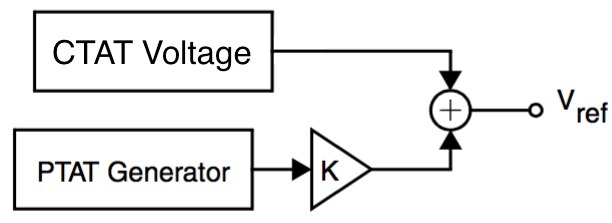
\includegraphics[scale=0.35]{photo/schema_principe}
   \end{minipage}\hfill
   \begin{minipage}[b]{0.5\linewidth}
      \centering 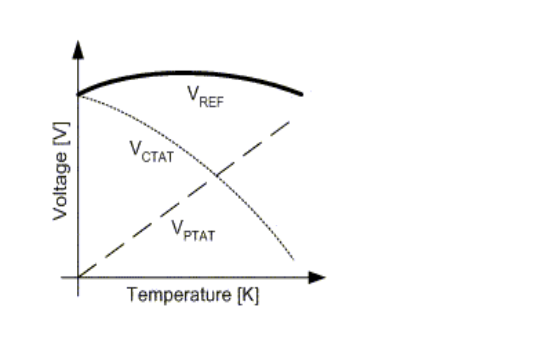
\includegraphics[scale=0.4]{photo/sum_crb}
   \end{minipage}
   \caption{General Bandgap Voltage Principle}
   \label{Gene_bandgap}
\end{figure}

Now, we need to find the component, or a characteristic that has a PTAT or CTAT behaviour. We are going to use the usual componenent, Bipolar and MOS transistor. In one hand, we can notice that the temperature coefficient of (evolution with respect to Temperature ) $V_{BE}$ is negative, as well as the $V_{GS}$ of a MOS transitor. In the other hand, we can observe that two bipolar or MOS transistor working at a unequal current densities create a voltage that is proportionnal to $U_T = \frac{kT}{q}$ therefore PTAT voltage (Positive Temperature Coefficient - TC).

The bandgap voltage reference will be used in different block, and for applications with low power consumption. The design will then take into account some specifications related to these applications. We can resume the main specifications of this project in the next table :

\begin{table}[h]
  \begin{center}
  \begin{tabular}{|c|c|c|c|} \hline
                                 & Typ & Maximum       & Minimum \\ \hline
    \textbf{Current Consumption} & $1~\mu$A & $3~\mu$A &   ---     \\ \hline
    \textbf{Power Supply Voltage}& 1.8 V    & 2 V      & 1.5 V \\ \hline \hline
    \textbf{Technology}          & \multicolumn{3}{c|}{UMC L180}  \\ \hline
  \end{tabular}
\end{center}
\caption{Voltage Reference Specifications}
\end{table}


\chapter{Generate a CTAT Voltage}
\section{Evolution of $V_{BE}$ with respect to temperature}

The base-emmiter voltage of a bipolar transistors or, more generally, the forward voltage of a pn-junction diode show a negative TC. For a bipolar device such as represented in the Fig. \ref{vbe_T} 

\begin{figure}[h]
  \begin{center}
    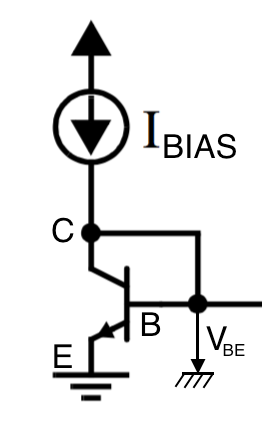
\includegraphics[scale=0.3]{photo/CTAT_VBE}
  \end{center}
  \caption{Base-emitter Voltage Context}
  \label{vbe_T}
\end{figure}

\begin{equation}
  V_{BE} = \frac{k_BT}{q} \cdot ln \left( \frac{I_C}{I_S} \right)
\end{equation}

With $I_S$, the saturation current which depend on the temperature through different characteristic ($n_i$, $\mu_0$) that depend differently of temperature. In a first calculation, we suppose that the collector current $I_C$ is independent of the temperature. After calculation (details on Appendix \ref{}) we obtain : 

\begin{equation}
 \frac{\partial V_{BE}}{\partial T} = \frac{V_{BE} - (4+m)U_T - E_g/q}{T}
 \label{DvbeDT}                        
\end{equation}

Where $m /approx -3/2$ a process parameter, $E_g /approx 1.12 eV $ the bandgap energy of silicon, $U_T = \frac{kT}{q}$ the thermal voltage. 
The equation \ref{DvbeDT}, reveal the dependence of the TC of $V_{BE}$ to the magnitude of $V_{BE}$ itself.
We then fix $V_BE \approx 700 mV $, $T \approx 300 K$ and we obtain $\frac{\partial V_{BE}}{\partial T} \approx -1.2 mV/ K$. In fact, in this part we limit our temperature analysis to the dependence to the first order of temperature which create a second order temperature dependence.


\newpage

\section{Bipolar Implementation in CMOS process}

The implementation of a bipolar transitor in a CMOS process used here process a lateral bipolar transistor which can be better controled and processed with a much better accuracy than the vertical bipolar. In fact, during the process, the depth of oxydation in the silicon is controlled with much more difficulty whereas the oxydation of a specific area is much more controled and processed with a better accuracy. We then use a lateral transistor, processed and layouted as in the Fig \ref{PNPCMOS} : 

\begin{figure}[h]
  \begin{center}
    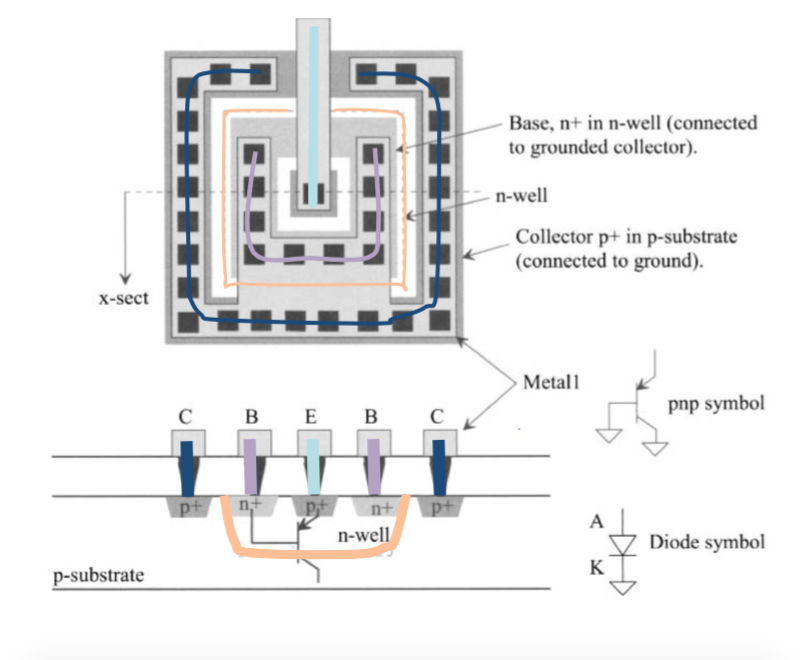
\includegraphics[scale=0.5]{photo/PNP_CMOS}
  \end{center}
  \caption{Layout of PNP Bipolar Transitor}
  \label{PNPCMOS}
\end{figure}

\chapter{Generate a PTAT Voltage}
\section{Using Base-emitter Voltage}

As said in the first chapter, we are going to use two bipolar transistor in two different current densities, and then the difference between their base-emitter voltage produce a voltage which is proportionnal to the thermal voltage, we then have a PTAT voltage.

We are going to use two branches with the same current I, and in one branch we are going to use n identical bipolar transitor and one bipolar transistor in the other branch ($I_{S2} = n I_{S}$ and $I_{S1} = I_{S}$).

\begin{align}
  \Delta V_{BE} & = V_{BE1} - V_{BE2} \\
              & = U_T ln \left( \frac{I_0}{I_{S1}}\right) - U_T ln \left( \frac{I_0}{I_{S2}}\right) \\
              & = \frac{kT}{q} \cdot ln(n)
\end{align}

\begin{figure}[h]
  \begin{center}
    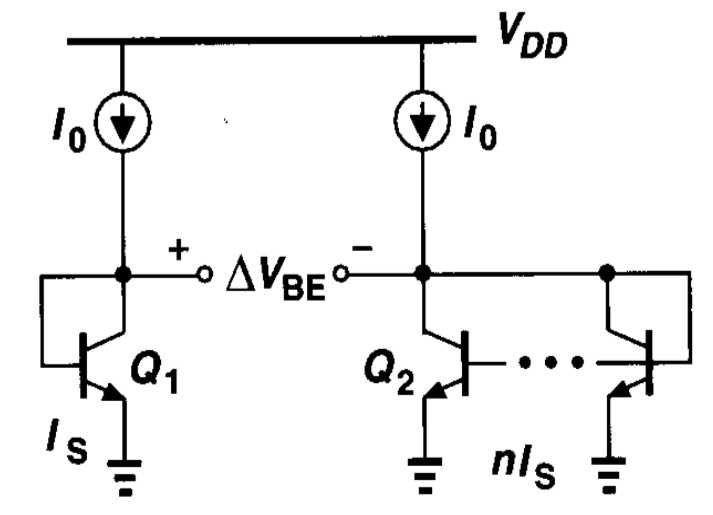
\includegraphics[scale=0.35]{photo/PTAT_1}
  \end{center}
  \caption{Generate a PTAT Voltage}
  \label{PTAT_1}
\end{figure}

\newpage

The precedent structure manipulate a differential voltage, the final idea is to add this voltage to a CTAT voltage which is not possible in a complete structure, so instead of generating a PTAT differential voltage, we generate a PTAT current which we can easily copy in another branch.

\begin{figure}[h]
  \begin{center}
    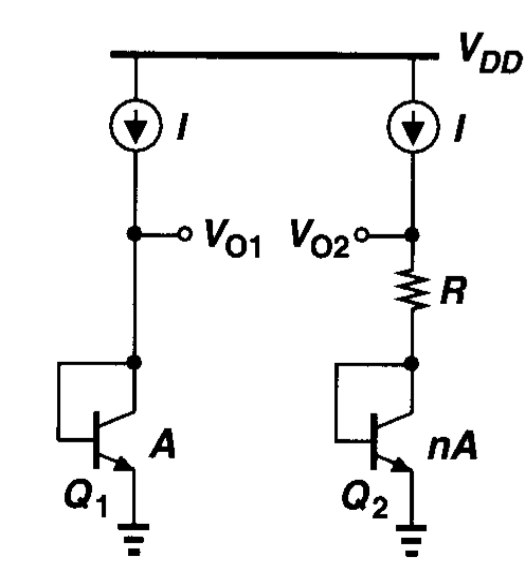
\includegraphics[scale=0.35]{photo/PTAT2}
  \end{center}
  \caption{Generate a PTAT Current}
\end{figure}

In this structure, we need also use a mechanism that will force $V_{O1} = V_{O2}$, we will use a operational amplifier with a high gain to force the two voltages to be equal.
\begin{align}
  V_{O1} & = V_{O2} \\
  V_{BE1}& = RI + V_{BE2} \\
  I      & = \frac{\Delta V_{BE}}{R} \\
         & = \frac{\frac{kT}{q}\cdot ln(n)}{R}
\end{align}

We obtain finally a PTAT current proportional to the thermal voltage that is easier to sum with a CTAT current or Voltage. Moreover we have two parameter n and R, that we can fix to cancel the negative temperature coefficient.

\section{Using Gate-source Voltage}

We use two transistor M1 and M2, which will operate in weak inversion with two different current densities. This region of operation have quasi the same way of variation than the bipolar transistor, whith a exponential dependence of the drain current with respect to the gate-source voltage.
\begin{align}
  I_{DS} & = I_{SPECs} \cdot \frac{W}{L} \cdot exp\left( q\frac{V_{gs}-V_t}{nkT} \right) \\
  I_{SPECs} & = 2 n \mu_{n} C_{ox} U_t^2
\end{align}

\newpage

In the same way, we use an Opamp to ensure that the two voltages $V_A$ $V_B$ are equal. We use the same current in the two branches, and we size the transistor M2 m times larger than M1, we then have :

\begin{align}
  V_{GS1} = & ~ n U_T \cdot ln\left( \frac{I_{DS1} \cdot L_1}{I_{SPECs} \cdot W_1} + V_{T0} \right) \\ 
  V_{GS2} = & ~ n U_T \cdot ln\left( \frac{I_{DS2} \cdot L_2}{I_{SPECs} \cdot W_2} + V_{T0} \right) \\
  \frac{W_2}{L_2} = & ~ m \cdot \frac{W_1}{L_1}
\end{align}

In the same logic we obtain a current $I_{R1}$ which is proportional to $\Delta V_{GS}$, in fact the final theoritical expression of $I_{R1} = \frac{\Delta V_{GS}}{R_1}$ with :

\begin{equation}
  \Delta V_{GS} = ~n~\frac{kT}{q}ln(m)
\end{equation} 

\begin{figure}[h]
  \begin{center}
    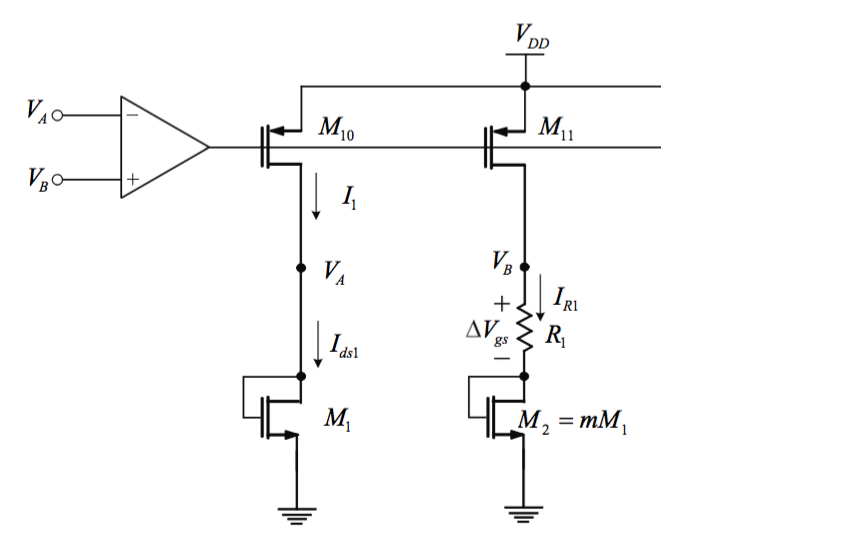
\includegraphics[scale=0.3]{photo/PTAT_MOS}
  \end{center}
  \caption{Generate a PTAT Current with MOS transistor}
  \label{PTAT_MOS}
\end{figure}

The final result is very similar to the bipolar "version", except that for the MOS version, $\Delta V_{GS}$ is proportionnal to the slope factor, except that this parameter is dependent of the temperature, the variation can be neglected for the dependence of the first order of temperature. 

\chapter{Bandgap Voltage}
\section{Current Source - Beta-Multiplier}

As we are limited to 3 $\mu A$ in current consumption, we are going to limit the current consumption in the current-source to the minimum. We decide then to produce a current of 100 nA that we are going to mirror in the different branches to generate a PTAT and a CTAT voltage. To generate this current, we are going the structure in the Fig \ref{beta_m} :

\begin{figure}[h]
  \begin{center}
    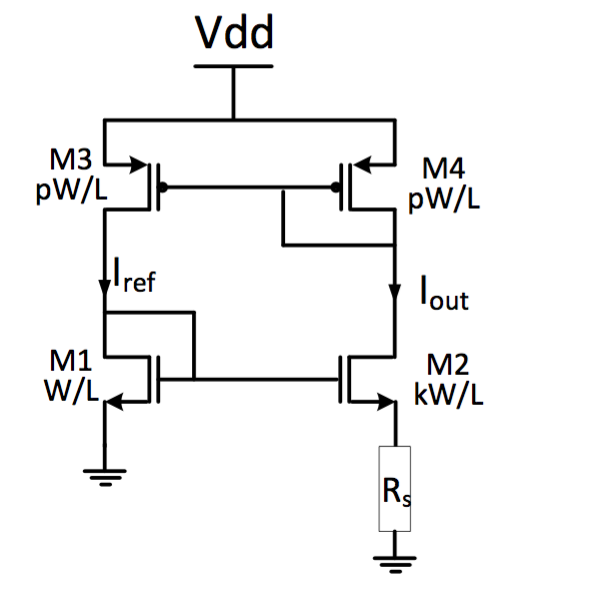
\includegraphics[scale=0.3]{photo/beta_multiplier}
  \end{center}
  \caption{Beta-Multiplier Current Source}
  \label{beta_m}
\end{figure}

For such low current, we use the two transistor M1 and M2 in weak inversion, and to obtain a good current mirror with respect to mismatch and have $I_{ref}$ quasi equal to $I_{out}$ we put the transistor M3 and M4 in strong inversion.

\begin{equation}
  I_{out} = I_{spec} \cdot exp \left( \frac{V_G - n V_S - V_{T0}}{n U_T}\right)
\end{equation}

If we apply this equation to the transitor M1 and M2, with M2 k times larger than M1, we have a simple equation :

\begin{equation}
  I_{out} = I_{ref} = \frac{U_T \cdot ln(k)}{R_S}
\end{equation}

\begin{table}[h]
  \begin{center}
  \begin{tabular}{|c|c|}\hline
    $W_1 = 4~\mu m$       & $L_1 = 180~ nm$ \\ \hline
    $W_2 =  16~ \mu m$       & $L_2 = 180~ nm$ \\ \hline
    $W_3 = W_4 = 5~ \mu m$ & $L_3 = L_4 = 250~ nm$  \\ \hline
    $W_5 = W_6 = 1~ \mu m$ & $L_5 = L_6 = 300~ nm$ \\ \hline
  \end{tabular}
\end{center}
\caption{Beta-Multiplier transitor dimension}
\end{table}



\section{Single Stage OTA}

\begin{figure}[h]
  \begin{center}
    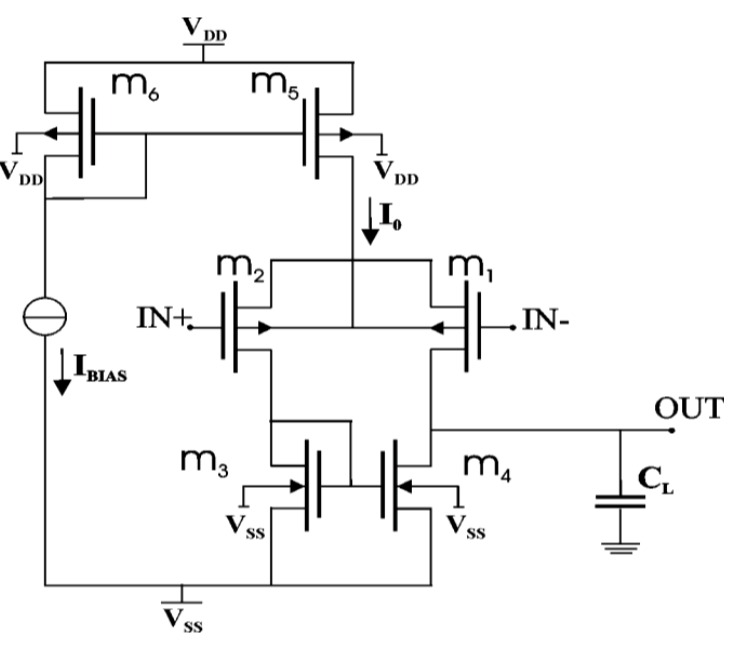
\includegraphics[scale=0.35]{photo/OTA_Pmos}
  \end{center}
  \caption{OTA with PMOS differential pair}
  \label{OTA}
\end{figure}

\begin{table}[h]
  \begin{center}
  \begin{tabular}{|c|c|}\hline
    $W_1 = W_2 = \mu m$ & $L_1 = L_2 = \mu m$  \\ \hline
    $W_3 = W_4 = \mu m$ & $L_3 = L_4 = \mu m$ \\ \hline
    $W_5 = \mu m$       & $L_5 = \mu m$ \\ \hline
  \end{tabular}
\end{center}
\caption{OTA transitor dimension}
\end{table}

\section{Overall circuits}
\subsection{Bandgap Voltage Reference}



\subsection{ Sub-1V Bandgap Current and Voltage Reference}



\chapter{Results after Simulation}
\section{Temperature Dependence}
\section{Dependence to VDD - PSRR}
\section{Simulation Post route}

\chapter*{Conclusion}
\addcontentsline{toc}{chapter}{Conclusion}


%%%%%%%%%%%%%%% Début de la gestion de l'annexe %%%%%%%%%%%%%%

\begin{appendices}
\chapter{Evolution of $V_{BE}$ with respect to temperature}

The details of the calculation of the dependence of $V_{BE}$ to temperature. We fisrt devellop the temperature dependence : 

\begin{align}
  V_{BE} & = \frac{k_BT}{q} \cdot ln \left( \frac{I_C}{I_S} \right) \\
  I_S ~   & \alpha ~ \mu ~ k T ~ n_i^2 \\
  \mu ~   & \alpha ~ \mu_0 ~ T^m \\
  n_i^2 ~ & \alpha~ T^3  \cdot  exp\left(\frac{E_g}{kT}\right)
\end{align}

With $\mu$ the mobility of the carriers, $n_i$ the intrinsic carrier concentration of silicon and $E_g~\approx 1.12 eV$ the bandgap energy of silicon.

We introduce a parameter b, which is a proprtionnality factor :

\begin{equation}
  I_S = b T^{4+m} \cdot exp\left(\frac{E_g}{kT}\right)
\end{equation}

Once we have devellop the expression with respect with T, we start to derivate the expression : 

\begin{equation}
    \frac{\partial V_{BE}}{\partial T} = \frac{\partial U_{T}}{\partial T}\cdot ln \left( \frac{I_C}{I_S} \right) + \frac{\partial I_{S}}{\partial T} \cdot \frac{U_T}{I_S}
\end{equation}

\begin{equation}
  \frac{\partial I_{S}}{\partial T} = b(4+m)T^{3+m}\cdot exp\left(\frac{E_g}{kT}\right) + bT^{4+m}\left(exp\left(\frac{E_g}{kT}\right)\right)\cdot \frac{E_g}{k T^{2}} 
\end{equation}

  
\begin{equation}
  \frac{U_T}{I_S} \frac{\partial I_{S}}{\partial T} = (4+m)\frac{U_T}{T} + \frac{E_g}{kT^2}\cdot U_T
\end{equation}

We obtain finally :

\begin{align}
  \frac{\partial V_{BE}}{\partial T} & = \frac{U_T}{T} ln \left( \frac{I_C}{I_S} \right) - (4+m)\frac{U_T}{T} - \frac{E_g}{kT^2}\cdot U_T \\
  \frac{\partial V_{BE}}{\partial T} & = \frac{V_{BE} - (4+m)U_T - E_g/q}{T}
\end{align}



\chapter{ ANNEXE B}
\chapter{ ANNEXE C}
\end{appendices}

%%%%%%%%%%%%%%%%%%%%%%%%%%%%%%%%%%%%%%%%%%%%%%%%%%%%%%%%%%%%



\end{document}
